%%%%%%%%%%%%%%%%%%%%%%%%%%%%%%%		CHAP 6		%%%%%%%%%%%%%%%%%%%%%%%%%%%%%%%

\chapter{Data analysis results}
\label{cha:5}

\textcolor{blue}{I feel like basing all this chapter upon the parameters variation.}
 
 Some results regarding the validity of the selection method, discussed in the previous chapter, are %
 presented here.

 Using the techniques described in the previous section, the selected data sets are %
 studied (see section~ref) in order to test the validity of the selection method proposed.
 The rate of cosmic is also evaluated, as well as the muon lifetime and the neutron yield %

\section{Cosmic background data}
\textcolor{blue}{The idea here is to compare expected muon rate with measured one.}

 High energy particles, mainly originated outside the Solar System and thus called %
 \emph{Cosmic Rays}, impact on the Earth's atmosphere and producing mesons, which in turn generate %
 secondary particle shower by decaying.
 The primary particles are about 99\,\% made of ionised nuclei (79\,\% protons, 19\,\% alphas, 2\,\% %
 heavier nuclei), while the remaining 1\,\% is mostly composed by electrons.
 The intensity of the nucleons in the energy range from several GeV to somewhat beyond 100 TeV %
 is given approximately by
 \begin{equation}
   \label{eq:cosmicI}
   I_N(E) \simeq \np{1.8e4} (\frac{E}{1~Gev})^{-\alpha}~\mathrm{\frac{nucleons}{m^2\,s\,sr\,Gev}}\,,
 \end{equation}
 where $E$ is the energy-per-nucleon, including rest mass energy, and $\alpha = \gamma +1 = \np{2.7}$ %
 is the differential spectral index of the cosmic ray flux, with $\gamma$ the integral spectral %
 index.

 Many are the secondary products reaching the sea level, among which muons, neutrinos, nucleons, and %
 electrons.
 The first two, muons and neutrinos, derive from the decay chain of charged mesons, while electrons %
 and photons originate in decays of neutral mesons.

 \begin{figure}[]
   \centering
   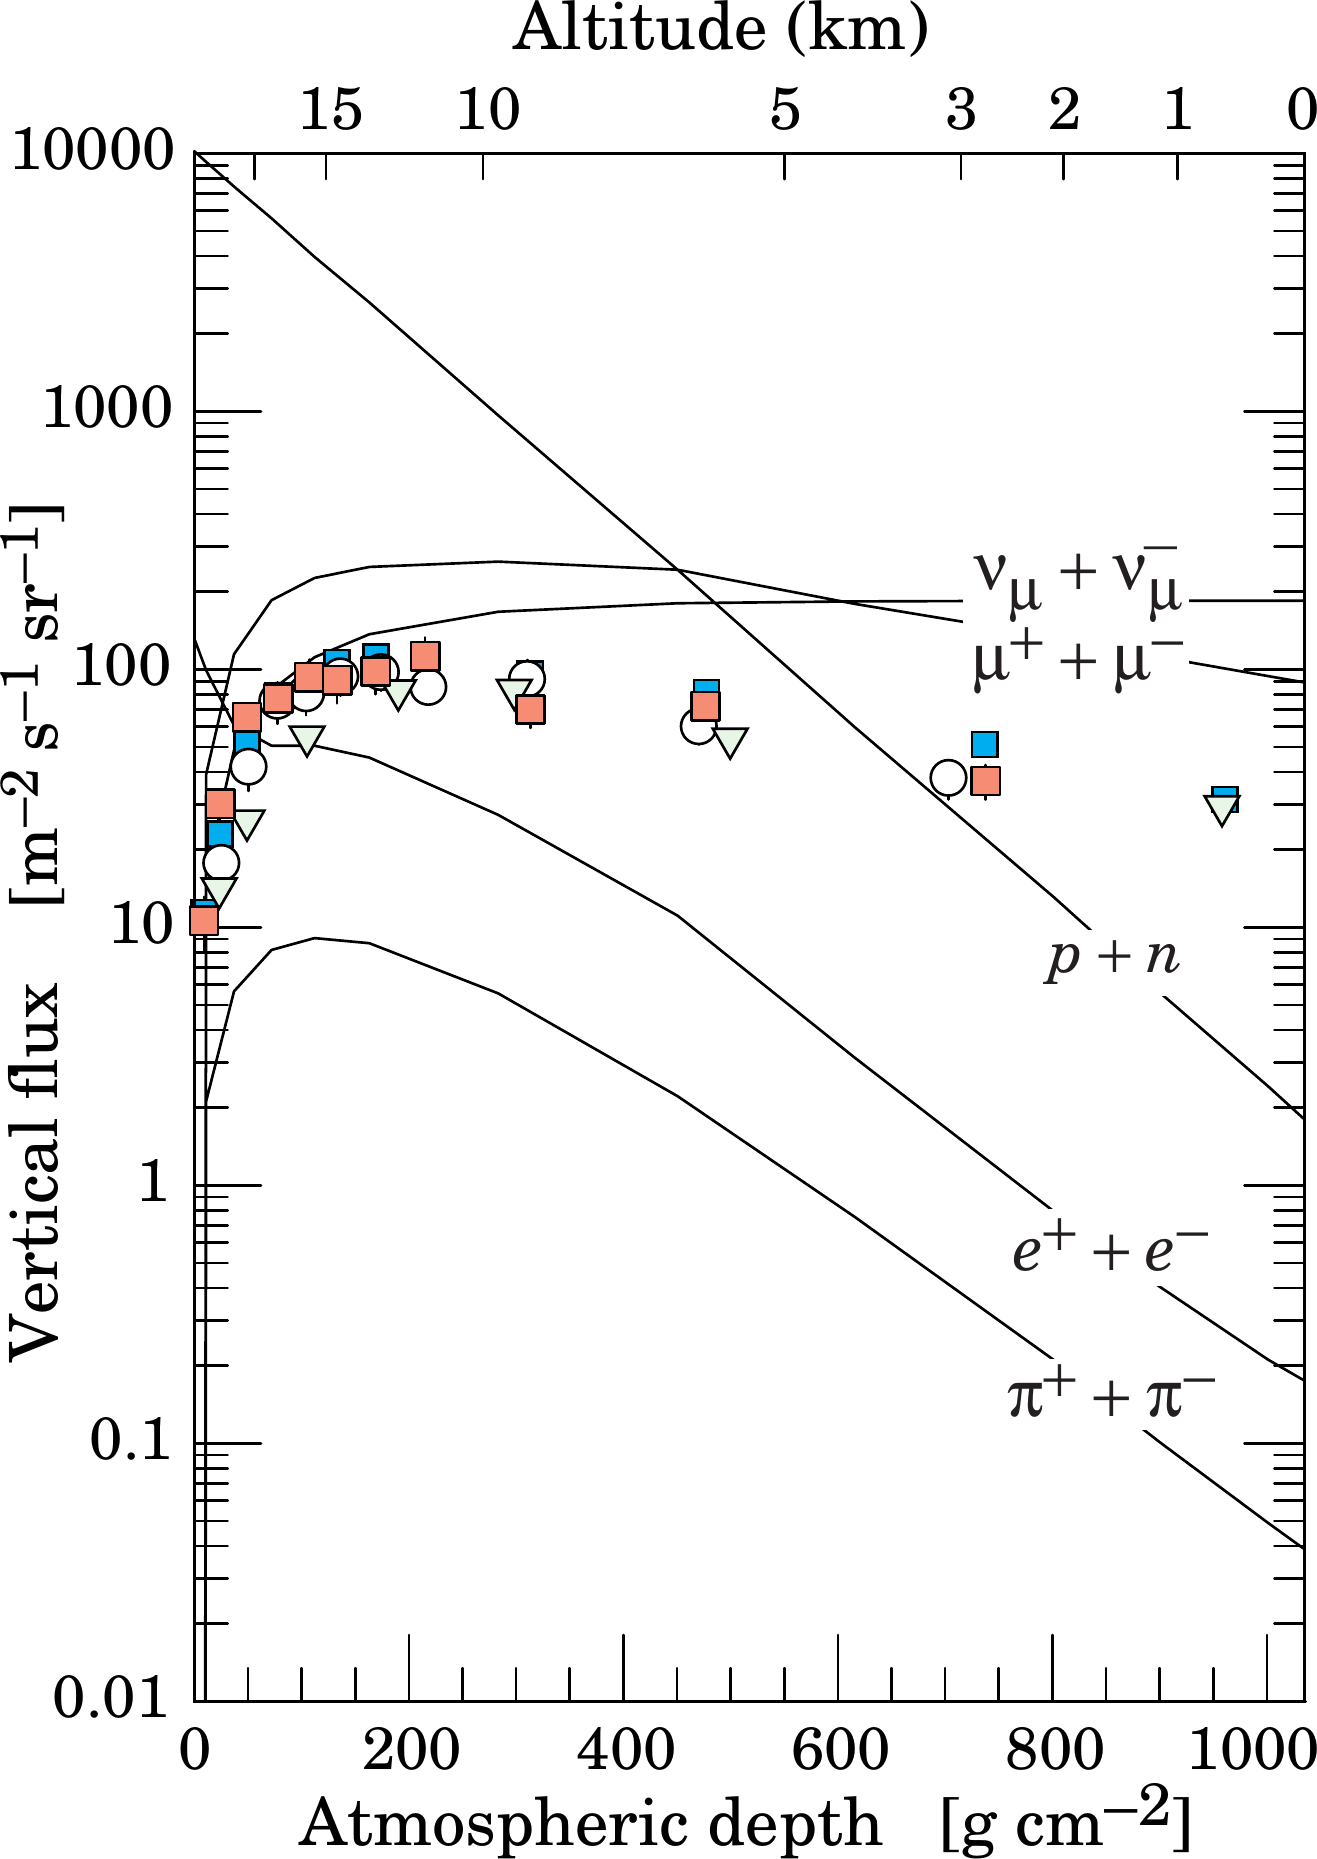
\includegraphics[scale=0.20]{pics/muonflux}
   \caption{Vertical fluxes of cosmic rays in the atmosphere with $E > 1$~GeV estimated %
     from the nucleon flux of Eq.~\ref{eq:cosmicI}. The points show measurements of negative muons %
     with 1 GeV from~ref[32–36].}
   \label{fig:muonflux}
 \end{figure}

 As Fig.~\ref{fig:muonflux} shows, muons are the most numerous charged particles at sea level.
 Muons lose energy to ionisation at a fairly constant rate of about 2~MeV per g/cm$^2$.
 Given that the vertical depth of the atmosphere is about 1000~g/cm$^2$, muons will lose about two~GeV %
 before reaching the ground. 
 The mean energy of muons at sea level is about four~GeV; therefore the mean energy at creation, %
 typically fifteen kilometres high, is probably near six~GeV.
 Their energy and angular distribution reflect a convolution of the production spectrum, %
 energy loss in the atmosphere, and decay. 
 The energy spectrum is almost flat below 1 GeV, steepens gradually to reflect the primary %
 spectrum in the 10$\div$100~GeV range, and steepens further at higher energies because pions %
 with $E_\pi > \epsilon_\pi$ tend to interact in the atmosphere before they decay, where %
 $\epsilon_\pi = 115$~GeV is the critical decay energy for pions.
 Asymptotically ($E_\mu \gg $ 1~TeV), the energy spectrum of atmospheric muons is one power %
 steeper than the primary spectrum. 
 The integral intensity of vertical muons above 1~GeV/c at sea level is nearly 70~m$^{-2}$s$^{-1}$sr$^{-1}$ %
 [41,42], with recent measurements [43–45] favouring a lower normalisation by 10-15\,\%.
 Another way to express this evaluation is the form 
 \begin{equation}
   \label{eq:muon:rate}
   I_0 \simeq 1~\mathrm{cm^{-2}min^{-1}} = \np{166.7}~\mathrm{m^{-2}Hz}\,,
 \end{equation}
 for horizontal detectors. 
 The overall angular distribution of muons at the ground is $\propto \cos 2\vartheta$, which is %
 characteristic of muons with $E_\mu \sim 3$~GeV. 
% At lower energy the angular distribution becomes increasingly steep, while at higher energy it flattens, %
% approaching a $\sec\vartheta$ distribution for $E_\mu \gg \epsilon_pi$ and $\vartheta < 70^\circ$.
 
 With the beam off, only cosmic rays and background leave a trace in the detector.
 Therefore runs 93 and 94 are useful to characterise the background.

 From Eq.~\ref{eq:ch_Eth}, every muon with an energy $E > \np{159.739}$~MeV can produce Cherenkov %
 radiation, given that the refractive index of water is $n = \np{1.33}$ and %
 the muon mass is \np{105.658}~MeV\footnote{The muon mass is known with an accuracy of order \np{e-8}. %
   According to the PDF, $m_\mu = \np{105.6583715} \pm \np{0.0000035}$~MeV.}.
 Since the average energy of the muon reaching the ground is well above the Cherenkov threshold, %
 the nominal flux at sea level can be used to evaluate the cosmic background rate.
 The water tank is placed eight meters below the surface, and it fits the hall's walls, hence only the top %
 area of the tank (slightly more than 7~m$^2$) could be taken in consideration.
 A rough estimation suggests that the number of muons reaching the detector is 
 \begin{equation}
   \label{eq:anniemuon}
   I \simeq 7~\mathrm{m^2}\,I_0 \simeq \np{1178.1}~Hz\,.
 \end{equation}

 From the runs selected\ldots


\section{Threshold dependence}

Three parameters of the Data Analysis software have been tuned so as to study the feedback %
of the rejection method.
The parameters are:
\begin{enumerate}
  \item Voltage threshold;
  \item Number of PMTs fired;
  \item Time rejection window.
\end{enumerate}

\textcolor{blue}{Loads of tables here: something about final size and zero-suppression,\ldots}
\subsection{Voltage}
\subsection{PMTs fired}
\subsection{Rejection window}

\section{Michel decay}
I've seen it, it could be a nice plot to place here. 

\section{Neutron yield}
No luck yet.
really not sure whether or not include this section.

\section{First MRD data}
TDC, could do some dummy analysis.
